% Created by tikzDevice version 0.12.3.1 on 2022-09-05 08:11:27
% !TEX encoding = UTF-8 Unicode
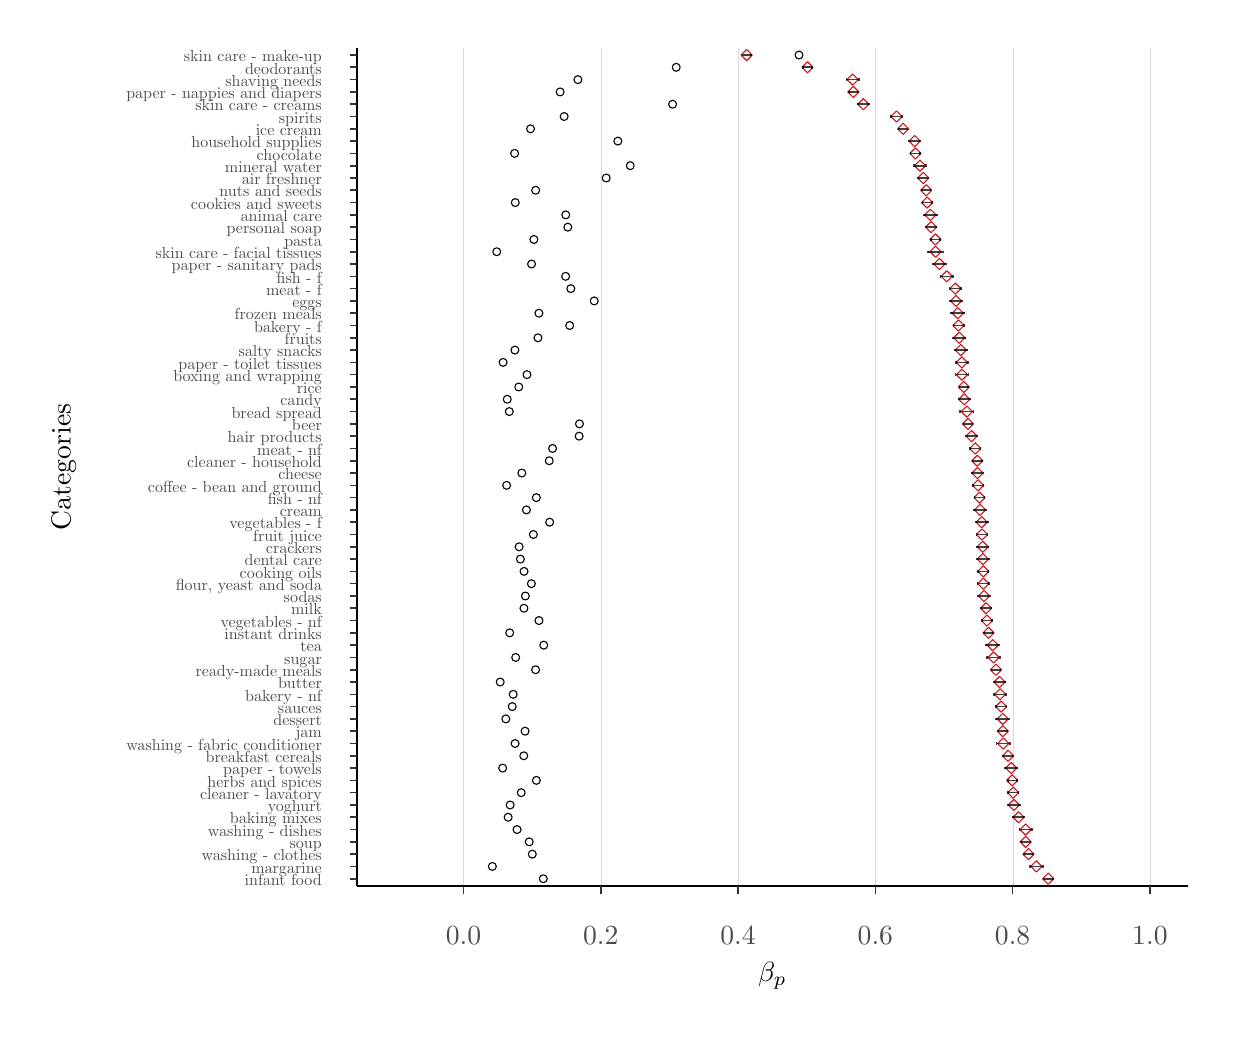
\begin{tikzpicture}[x=1pt,y=1pt]
\definecolor{fillColor}{RGB}{255,255,255}
\path[use as bounding box,fill=fillColor,fill opacity=0.00] (0,0) rectangle (433.62,361.35);
\begin{scope}
\path[clip] (  0.00,  0.00) rectangle (433.62,361.35);
\definecolor{drawColor}{RGB}{255,255,255}
\definecolor{fillColor}{RGB}{255,255,255}

\path[draw=drawColor,line width= 0.6pt,line join=round,line cap=round,fill=fillColor] (  0.00,  0.00) rectangle (433.62,361.35);
\end{scope}
\begin{scope}
\path[clip] (119.04, 51.15) rectangle (419.17,354.12);
\definecolor{drawColor}{RGB}{255,255,255}

\path[draw=drawColor,line width= 0.3pt,line join=round] (132.68, 51.15) --
	(132.68,354.12);

\path[draw=drawColor,line width= 0.3pt,line join=round] (182.29, 51.15) --
	(182.29,354.12);

\path[draw=drawColor,line width= 0.3pt,line join=round] (231.90, 51.15) --
	(231.90,354.12);

\path[draw=drawColor,line width= 0.3pt,line join=round] (281.51, 51.15) --
	(281.51,354.12);

\path[draw=drawColor,line width= 0.3pt,line join=round] (331.11, 51.15) --
	(331.11,354.12);

\path[draw=drawColor,line width= 0.3pt,line join=round] (380.72, 51.15) --
	(380.72,354.12);
\definecolor{drawColor}{gray}{0.85}

\path[draw=drawColor,line width= 0.1pt,line join=round] (157.49, 51.15) --
	(157.49,354.12);

\path[draw=drawColor,line width= 0.1pt,line join=round] (207.09, 51.15) --
	(207.09,354.12);

\path[draw=drawColor,line width= 0.1pt,line join=round] (256.70, 51.15) --
	(256.70,354.12);

\path[draw=drawColor,line width= 0.1pt,line join=round] (306.31, 51.15) --
	(306.31,354.12);

\path[draw=drawColor,line width= 0.1pt,line join=round] (355.92, 51.15) --
	(355.92,354.12);

\path[draw=drawColor,line width= 0.1pt,line join=round] (405.52, 51.15) --
	(405.52,354.12);
\definecolor{drawColor}{RGB}{0,0,0}

\path[draw=drawColor,line width= 0.4pt,line join=round,line cap=round] (209.06,307.03) circle (  1.43);

\path[draw=drawColor,line width= 0.4pt,line join=round,line cap=round] (194.43,293.71) circle (  1.43);

\path[draw=drawColor,line width= 0.4pt,line join=round,line cap=round] (195.86,253.73) circle (  1.43);

\path[draw=drawColor,line width= 0.4pt,line join=round,line cap=round] (175.43,120.45) circle (  1.43);

\path[draw=drawColor,line width= 0.4pt,line join=round,line cap=round] (173.61, 76.03) circle (  1.43);

\path[draw=drawColor,line width= 0.4pt,line join=round,line cap=round] (199.39,218.19) circle (  1.43);

\path[draw=drawColor,line width= 0.4pt,line join=round,line cap=round] (180.43,235.96) circle (  1.43);

\path[draw=drawColor,line width= 0.4pt,line join=round,line cap=round] (174.03,222.63) circle (  1.43);

\path[draw=drawColor,line width= 0.4pt,line join=round,line cap=round] (179.26, 98.24) circle (  1.43);

\path[draw=drawColor,line width= 0.4pt,line join=round,line cap=round] (170.75,124.90) circle (  1.43);

\path[draw=drawColor,line width= 0.4pt,line join=round,line cap=round] (173.29,227.07) circle (  1.43);

\path[draw=drawColor,line width= 0.4pt,line join=round,line cap=round] (178.55,200.42) circle (  1.43);

\path[draw=drawColor,line width= 0.4pt,line join=round,line cap=round] (175.96,315.92) circle (  1.43);

\path[draw=drawColor,line width= 0.4pt,line join=round,line cap=round] (188.47,204.86) circle (  1.43);

\path[draw=drawColor,line width= 0.4pt,line join=round,line cap=round] (178.34, 84.92) circle (  1.43);

\path[draw=drawColor,line width= 0.4pt,line join=round,line cap=round] (173.07,195.97) circle (  1.43);

\path[draw=drawColor,line width= 0.4pt,line join=round,line cap=round] (176.19,298.15) circle (  1.43);

\path[draw=drawColor,line width= 0.4pt,line join=round,line cap=round] (179.36,164.88) circle (  1.43);

\path[draw=drawColor,line width= 0.4pt,line join=round,line cap=round] (177.58,173.76) circle (  1.43);

\path[draw=drawColor,line width= 0.4pt,line join=round,line cap=round] (180.22,187.09) circle (  1.43);

\path[draw=drawColor,line width= 0.4pt,line join=round,line cap=round] (178.04,169.32) circle (  1.43);

\path[draw=drawColor,line width= 0.4pt,line join=round,line cap=round] (234.35,347.02) circle (  1.43);

\path[draw=drawColor,line width= 0.4pt,line join=round,line cap=round] (172.78,111.57) circle (  1.43);

\path[draw=drawColor,line width= 0.4pt,line join=round,line cap=round] (204.72,262.61) circle (  1.43);

\path[draw=drawColor,line width= 0.4pt,line join=round,line cap=round] (194.39,271.49) circle (  1.43);

\path[draw=drawColor,line width= 0.4pt,line join=round,line cap=round] (183.80,191.53) circle (  1.43);

\path[draw=drawColor,line width= 0.4pt,line join=round,line cap=round] (182.01,160.44) circle (  1.43);

\path[draw=drawColor,line width= 0.4pt,line join=round,line cap=round] (184.74,258.17) circle (  1.43);

\path[draw=drawColor,line width= 0.4pt,line join=round,line cap=round] (182.73,178.21) circle (  1.43);

\path[draw=drawColor,line width= 0.4pt,line join=round,line cap=round] (184.39,249.28) circle (  1.43);

\path[draw=drawColor,line width= 0.4pt,line join=round,line cap=round] (199.27,213.74) circle (  1.43);

\path[draw=drawColor,line width= 0.4pt,line join=round,line cap=round] (183.82, 89.36) circle (  1.43);

\path[draw=drawColor,line width= 0.4pt,line join=round,line cap=round] (213.26,320.36) circle (  1.43);

\path[draw=drawColor,line width= 0.4pt,line join=round,line cap=round] (181.71,324.80) circle (  1.43);

\path[draw=drawColor,line width= 0.4pt,line join=round,line cap=round] (186.32, 53.82) circle (  1.43);

\path[draw=drawColor,line width= 0.4pt,line join=round,line cap=round] (174.18,142.67) circle (  1.43);

\path[draw=drawColor,line width= 0.4pt,line join=round,line cap=round] (179.73,107.13) circle (  1.43);

\path[draw=drawColor,line width= 0.4pt,line join=round,line cap=round] (167.91, 58.26) circle (  1.43);

\path[draw=drawColor,line width= 0.4pt,line join=round,line cap=round] (196.26,267.05) circle (  1.43);

\path[draw=drawColor,line width= 0.4pt,line join=round,line cap=round] (189.67,209.30) circle (  1.43);

\path[draw=drawColor,line width= 0.4pt,line join=round,line cap=round] (179.32,151.55) circle (  1.43);

\path[draw=drawColor,line width= 0.4pt,line join=round,line cap=round] (217.74,311.48) circle (  1.43);

\path[draw=drawColor,line width= 0.4pt,line join=round,line cap=round] (183.55,302.59) circle (  1.43);

\path[draw=drawColor,line width= 0.4pt,line join=round,line cap=round] (192.41,338.13) circle (  1.43);

\path[draw=drawColor,line width= 0.4pt,line join=round,line cap=round] (182.07,275.94) circle (  1.43);

\path[draw=drawColor,line width= 0.4pt,line join=round,line cap=round] (171.80,240.40) circle (  1.43);

\path[draw=drawColor,line width= 0.4pt,line join=round,line cap=round] (171.64, 93.80) circle (  1.43);

\path[draw=drawColor,line width= 0.4pt,line join=round,line cap=round] (182.93,284.82) circle (  1.43);

\path[draw=drawColor,line width= 0.4pt,line join=round,line cap=round] (195.18,289.26) circle (  1.43);

\path[draw=drawColor,line width= 0.4pt,line join=round,line cap=round] (183.53,129.34) circle (  1.43);

\path[draw=drawColor,line width= 0.4pt,line join=round,line cap=round] (177.45,231.51) circle (  1.43);

\path[draw=drawColor,line width= 0.4pt,line join=round,line cap=round] (176.06,244.84) circle (  1.43);

\path[draw=drawColor,line width= 0.4pt,line join=round,line cap=round] (175.09,116.01) circle (  1.43);

\path[draw=drawColor,line width= 0.4pt,line join=round,line cap=round] (198.82,342.57) circle (  1.43);

\path[draw=drawColor,line width= 0.4pt,line join=round,line cap=round] (233.04,333.69) circle (  1.43);

\path[draw=drawColor,line width= 0.4pt,line join=round,line cap=round] (169.50,280.38) circle (  1.43);

\path[draw=drawColor,line width= 0.4pt,line join=round,line cap=round] (278.72,351.46) circle (  1.43);

\path[draw=drawColor,line width= 0.4pt,line join=round,line cap=round] (179.85,155.99) circle (  1.43);

\path[draw=drawColor,line width= 0.4pt,line join=round,line cap=round] (181.23, 67.15) circle (  1.43);

\path[draw=drawColor,line width= 0.4pt,line join=round,line cap=round] (193.85,329.25) circle (  1.43);

\path[draw=drawColor,line width= 0.4pt,line join=round,line cap=round] (176.34,133.78) circle (  1.43);

\path[draw=drawColor,line width= 0.4pt,line join=round,line cap=round] (186.48,138.22) circle (  1.43);

\path[draw=drawColor,line width= 0.4pt,line join=round,line cap=round] (188.62,182.65) circle (  1.43);

\path[draw=drawColor,line width= 0.4pt,line join=round,line cap=round] (184.75,147.11) circle (  1.43);

\path[draw=drawColor,line width= 0.4pt,line join=round,line cap=round] (182.34, 62.70) circle (  1.43);

\path[draw=drawColor,line width= 0.4pt,line join=round,line cap=round] (176.84, 71.59) circle (  1.43);

\path[draw=drawColor,line width= 0.4pt,line join=round,line cap=round] (176.12,102.69) circle (  1.43);

\path[draw=drawColor,line width= 0.4pt,line join=round,line cap=round] (174.34, 80.47) circle (  1.43);
\definecolor{drawColor}{RGB}{203,24,29}

\path[draw=drawColor,line width= 0.4pt,line join=round,line cap=round] (321.59,307.03) --
	(323.61,309.05) --
	(325.63,307.03) --
	(323.61,305.02) --
	cycle;

\path[draw=drawColor,line width= 0.4pt,line join=round,line cap=round] (324.17,293.71) --
	(326.19,295.72) --
	(328.21,293.71) --
	(326.19,291.69) --
	cycle;

\path[draw=drawColor,line width= 0.4pt,line join=round,line cap=round] (334.34,253.73) --
	(336.36,255.74) --
	(338.38,253.73) --
	(336.36,251.71) --
	cycle;

\path[draw=drawColor,line width= 0.4pt,line join=round,line cap=round] (349.35,120.45) --
	(351.36,122.47) --
	(353.38,120.45) --
	(351.36,118.44) --
	cycle;

\path[draw=drawColor,line width= 0.4pt,line join=round,line cap=round] (356.05, 76.03) --
	(358.06, 78.05) --
	(360.08, 76.03) --
	(358.06, 74.01) --
	cycle;

\path[draw=drawColor,line width= 0.4pt,line join=round,line cap=round] (337.76,218.19) --
	(339.78,220.20) --
	(341.79,218.19) --
	(339.78,216.17) --
	cycle;

\path[draw=drawColor,line width= 0.4pt,line join=round,line cap=round] (335.59,235.96) --
	(337.61,237.97) --
	(339.63,235.96) --
	(337.61,233.94) --
	cycle;

\path[draw=drawColor,line width= 0.4pt,line join=round,line cap=round] (337.36,222.63) --
	(339.38,224.65) --
	(341.40,222.63) --
	(339.38,220.61) --
	cycle;

\path[draw=drawColor,line width= 0.4pt,line join=round,line cap=round] (352.25, 98.24) --
	(354.26,100.26) --
	(356.28, 98.24) --
	(354.26, 96.23) --
	cycle;

\path[draw=drawColor,line width= 0.4pt,line join=round,line cap=round] (349.18,124.90) --
	(351.19,126.91) --
	(353.21,124.90) --
	(351.19,122.88) --
	cycle;

\path[draw=drawColor,line width= 0.4pt,line join=round,line cap=round] (336.43,227.07) --
	(338.45,229.09) --
	(340.47,227.07) --
	(338.45,225.05) --
	cycle;

\path[draw=drawColor,line width= 0.4pt,line join=round,line cap=round] (341.22,200.42) --
	(343.23,202.43) --
	(345.25,200.42) --
	(343.23,198.40) --
	cycle;

\path[draw=drawColor,line width= 0.4pt,line join=round,line cap=round] (318.77,315.92) --
	(320.79,317.94) --
	(322.81,315.92) --
	(320.79,313.90) --
	cycle;

\path[draw=drawColor,line width= 0.4pt,line join=round,line cap=round] (341.14,204.86) --
	(343.16,206.88) --
	(345.18,204.86) --
	(343.16,202.84) --
	cycle;

\path[draw=drawColor,line width= 0.4pt,line join=round,line cap=round] (354.10, 84.92) --
	(356.12, 86.93) --
	(358.13, 84.92) --
	(356.12, 82.90) --
	cycle;

\path[draw=drawColor,line width= 0.4pt,line join=round,line cap=round] (341.40,195.97) --
	(343.42,197.99) --
	(345.44,195.97) --
	(343.42,193.96) --
	cycle;

\path[draw=drawColor,line width= 0.4pt,line join=round,line cap=round] (322.99,298.15) --
	(325.01,300.17) --
	(327.03,298.15) --
	(325.01,296.13) --
	cycle;

\path[draw=drawColor,line width= 0.4pt,line join=round,line cap=round] (343.30,164.88) --
	(345.31,166.90) --
	(347.33,164.88) --
	(345.31,162.86) --
	cycle;

\path[draw=drawColor,line width= 0.4pt,line join=round,line cap=round] (343.08,173.76) --
	(345.10,175.78) --
	(347.11,173.76) --
	(345.10,171.75) --
	cycle;

\path[draw=drawColor,line width= 0.4pt,line join=round,line cap=round] (342.15,187.09) --
	(344.17,189.11) --
	(346.18,187.09) --
	(344.17,185.07) --
	cycle;

\path[draw=drawColor,line width= 0.4pt,line join=round,line cap=round] (343.13,169.32) --
	(345.15,171.34) --
	(347.17,169.32) --
	(345.15,167.30) --
	cycle;

\path[draw=drawColor,line width= 0.4pt,line join=round,line cap=round] (279.78,347.02) --
	(281.79,349.03) --
	(283.81,347.02) --
	(281.79,345.00) --
	cycle;

\path[draw=drawColor,line width= 0.4pt,line join=round,line cap=round] (350.33,111.57) --
	(352.35,113.59) --
	(354.37,111.57) --
	(352.35,109.55) --
	cycle;

\path[draw=drawColor,line width= 0.4pt,line join=round,line cap=round] (333.44,262.61) --
	(335.46,264.63) --
	(337.48,262.61) --
	(335.46,260.59) --
	cycle;

\path[draw=drawColor,line width= 0.4pt,line join=round,line cap=round] (330.08,271.49) --
	(332.10,273.51) --
	(334.12,271.49) --
	(332.10,269.48) --
	cycle;

\path[draw=drawColor,line width= 0.4pt,line join=round,line cap=round] (341.92,191.53) --
	(343.94,193.55) --
	(345.96,191.53) --
	(343.94,189.51) --
	cycle;

\path[draw=drawColor,line width= 0.4pt,line join=round,line cap=round] (343.31,160.44) --
	(345.33,162.45) --
	(347.35,160.44) --
	(345.33,158.42) --
	cycle;

\path[draw=drawColor,line width= 0.4pt,line join=round,line cap=round] (334.08,258.17) --
	(336.10,260.19) --
	(338.12,258.17) --
	(336.10,256.15) --
	cycle;

\path[draw=drawColor,line width= 0.4pt,line join=round,line cap=round] (342.82,178.21) --
	(344.84,180.22) --
	(346.86,178.21) --
	(344.84,176.19) --
	cycle;

\path[draw=drawColor,line width= 0.4pt,line join=round,line cap=round] (334.62,249.28) --
	(336.64,251.30) --
	(338.66,249.28) --
	(336.64,247.27) --
	cycle;

\path[draw=drawColor,line width= 0.4pt,line join=round,line cap=round] (339.06,213.74) --
	(341.07,215.76) --
	(343.09,213.74) --
	(341.07,211.73) --
	cycle;

\path[draw=drawColor,line width= 0.4pt,line join=round,line cap=round] (353.75, 89.36) --
	(355.77, 91.38) --
	(357.79, 89.36) --
	(355.77, 87.34) --
	cycle;

\path[draw=drawColor,line width= 0.4pt,line join=round,line cap=round] (318.49,320.36) --
	(320.50,322.38) --
	(322.52,320.36) --
	(320.50,318.34) --
	cycle;

\path[draw=drawColor,line width= 0.4pt,line join=round,line cap=round] (314.34,324.80) --
	(316.36,326.82) --
	(318.38,324.80) --
	(316.36,322.79) --
	cycle;

\path[draw=drawColor,line width= 0.4pt,line join=round,line cap=round] (366.75, 53.82) --
	(368.77, 55.84) --
	(370.78, 53.82) --
	(368.77, 51.80) --
	cycle;

\path[draw=drawColor,line width= 0.4pt,line join=round,line cap=round] (345.18,142.67) --
	(347.20,144.68) --
	(349.21,142.67) --
	(347.20,140.65) --
	cycle;

\path[draw=drawColor,line width= 0.4pt,line join=round,line cap=round] (350.35,107.13) --
	(352.36,109.14) --
	(354.38,107.13) --
	(352.36,105.11) --
	cycle;

\path[draw=drawColor,line width= 0.4pt,line join=round,line cap=round] (362.46, 58.26) --
	(364.48, 60.28) --
	(366.49, 58.26) --
	(364.48, 56.24) --
	cycle;

\path[draw=drawColor,line width= 0.4pt,line join=round,line cap=round] (333.16,267.05) --
	(335.18,269.07) --
	(337.20,267.05) --
	(335.18,265.04) --
	cycle;

\path[draw=drawColor,line width= 0.4pt,line join=round,line cap=round] (340.38,209.30) --
	(342.40,211.32) --
	(344.42,209.30) --
	(342.40,207.28) --
	cycle;

\path[draw=drawColor,line width= 0.4pt,line join=round,line cap=round] (344.30,151.55) --
	(346.32,153.57) --
	(348.34,151.55) --
	(346.32,149.53) --
	cycle;

\path[draw=drawColor,line width= 0.4pt,line join=round,line cap=round] (320.42,311.48) --
	(322.44,313.49) --
	(324.46,311.48) --
	(322.44,309.46) --
	cycle;

\path[draw=drawColor,line width= 0.4pt,line join=round,line cap=round] (322.69,302.59) --
	(324.71,304.61) --
	(326.72,302.59) --
	(324.71,300.57) --
	cycle;

\path[draw=drawColor,line width= 0.4pt,line join=round,line cap=round] (296.34,338.13) --
	(298.35,340.15) --
	(300.37,338.13) --
	(298.35,336.11) --
	cycle;

\path[draw=drawColor,line width= 0.4pt,line join=round,line cap=round] (327.45,275.94) --
	(329.47,277.95) --
	(331.49,275.94) --
	(329.47,273.92) --
	cycle;

\path[draw=drawColor,line width= 0.4pt,line join=round,line cap=round] (335.53,240.40) --
	(337.55,242.42) --
	(339.57,240.40) --
	(337.55,238.38) --
	cycle;

\path[draw=drawColor,line width= 0.4pt,line join=round,line cap=round] (353.40, 93.80) --
	(355.42, 95.82) --
	(357.43, 93.80) --
	(355.42, 91.78) --
	cycle;

\path[draw=drawColor,line width= 0.4pt,line join=round,line cap=round] (325.97,284.82) --
	(327.99,286.84) --
	(330.01,284.82) --
	(327.99,282.80) --
	cycle;

\path[draw=drawColor,line width= 0.4pt,line join=round,line cap=round] (324.46,289.26) --
	(326.47,291.28) --
	(328.49,289.26) --
	(326.47,287.25) --
	cycle;

\path[draw=drawColor,line width= 0.4pt,line join=round,line cap=round] (347.87,129.34) --
	(349.89,131.36) --
	(351.91,129.34) --
	(349.89,127.32) --
	cycle;

\path[draw=drawColor,line width= 0.4pt,line join=round,line cap=round] (336.23,231.51) --
	(338.24,233.53) --
	(340.26,231.51) --
	(338.24,229.50) --
	cycle;

\path[draw=drawColor,line width= 0.4pt,line join=round,line cap=round] (335.16,244.84) --
	(337.18,246.86) --
	(339.19,244.84) --
	(337.18,242.82) --
	cycle;

\path[draw=drawColor,line width= 0.4pt,line join=round,line cap=round] (349.76,116.01) --
	(351.78,118.03) --
	(353.80,116.01) --
	(351.78,113.99) --
	cycle;

\path[draw=drawColor,line width= 0.4pt,line join=round,line cap=round] (296.09,342.57) --
	(298.11,344.59) --
	(300.13,342.57) --
	(298.11,340.56) --
	cycle;

\path[draw=drawColor,line width= 0.4pt,line join=round,line cap=round] (299.96,333.69) --
	(301.97,335.71) --
	(303.99,333.69) --
	(301.97,331.67) --
	cycle;

\path[draw=drawColor,line width= 0.4pt,line join=round,line cap=round] (326.04,280.38) --
	(328.06,282.40) --
	(330.07,280.38) --
	(328.06,278.36) --
	cycle;

\path[draw=drawColor,line width= 0.4pt,line join=round,line cap=round] (257.77,351.46) --
	(259.79,353.48) --
	(261.81,351.46) --
	(259.79,349.44) --
	cycle;

\path[draw=drawColor,line width= 0.4pt,line join=round,line cap=round] (343.54,155.99) --
	(345.56,158.01) --
	(347.58,155.99) --
	(345.56,153.98) --
	cycle;

\path[draw=drawColor,line width= 0.4pt,line join=round,line cap=round] (358.62, 67.15) --
	(360.63, 69.16) --
	(362.65, 67.15) --
	(360.63, 65.13) --
	cycle;

\path[draw=drawColor,line width= 0.4pt,line join=round,line cap=round] (311.94,329.25) --
	(313.95,331.26) --
	(315.97,329.25) --
	(313.95,327.23) --
	cycle;

\path[draw=drawColor,line width= 0.4pt,line join=round,line cap=round] (347.03,133.78) --
	(349.04,135.80) --
	(351.06,133.78) --
	(349.04,131.76) --
	cycle;

\path[draw=drawColor,line width= 0.4pt,line join=round,line cap=round] (346.70,138.22) --
	(348.72,140.24) --
	(350.74,138.22) --
	(348.72,136.21) --
	cycle;

\path[draw=drawColor,line width= 0.4pt,line join=round,line cap=round] (342.72,182.65) --
	(344.74,184.67) --
	(346.76,182.65) --
	(344.74,180.63) --
	cycle;

\path[draw=drawColor,line width= 0.4pt,line join=round,line cap=round] (344.61,147.11) --
	(346.62,149.13) --
	(348.64,147.11) --
	(346.62,145.09) --
	cycle;

\path[draw=drawColor,line width= 0.4pt,line join=round,line cap=round] (359.63, 62.70) --
	(361.65, 64.72) --
	(363.66, 62.70) --
	(361.65, 60.69) --
	cycle;

\path[draw=drawColor,line width= 0.4pt,line join=round,line cap=round] (358.59, 71.59) --
	(360.60, 73.61) --
	(362.62, 71.59) --
	(360.60, 69.57) --
	cycle;

\path[draw=drawColor,line width= 0.4pt,line join=round,line cap=round] (350.50,102.69) --
	(352.51,104.70) --
	(354.53,102.69) --
	(352.51,100.67) --
	cycle;

\path[draw=drawColor,line width= 0.4pt,line join=round,line cap=round] (354.34, 80.47) --
	(356.36, 82.49) --
	(358.38, 80.47) --
	(356.36, 78.46) --
	cycle;
\definecolor{drawColor}{RGB}{0,0,0}

\path[draw=drawColor,draw opacity=0.75,line width= 0.6pt,line join=round] (325.50,306.59) --
	(325.50,307.48);

\path[draw=drawColor,draw opacity=0.75,line width= 0.6pt,line join=round] (325.50,307.03) --
	(321.72,307.03);

\path[draw=drawColor,draw opacity=0.75,line width= 0.6pt,line join=round] (321.72,306.59) --
	(321.72,307.48);

\path[draw=drawColor,draw opacity=0.75,line width= 0.6pt,line join=round] (328.51,293.26) --
	(328.51,294.15);

\path[draw=drawColor,draw opacity=0.75,line width= 0.6pt,line join=round] (328.51,293.71) --
	(323.87,293.71);

\path[draw=drawColor,draw opacity=0.75,line width= 0.6pt,line join=round] (323.87,293.26) --
	(323.87,294.15);

\path[draw=drawColor,draw opacity=0.75,line width= 0.6pt,line join=round] (338.22,253.28) --
	(338.22,254.17);

\path[draw=drawColor,draw opacity=0.75,line width= 0.6pt,line join=round] (338.22,253.73) --
	(334.50,253.73);

\path[draw=drawColor,draw opacity=0.75,line width= 0.6pt,line join=round] (334.50,253.28) --
	(334.50,254.17);

\path[draw=drawColor,draw opacity=0.75,line width= 0.6pt,line join=round] (353.61,120.01) --
	(353.61,120.90);

\path[draw=drawColor,draw opacity=0.75,line width= 0.6pt,line join=round] (353.61,120.45) --
	(349.12,120.45);

\path[draw=drawColor,draw opacity=0.75,line width= 0.6pt,line join=round] (349.12,120.01) --
	(349.12,120.90);

\path[draw=drawColor,draw opacity=0.75,line width= 0.6pt,line join=round] (360.06, 75.59) --
	(360.06, 76.48);

\path[draw=drawColor,draw opacity=0.75,line width= 0.6pt,line join=round] (360.06, 76.03) --
	(356.07, 76.03);

\path[draw=drawColor,draw opacity=0.75,line width= 0.6pt,line join=round] (356.07, 75.59) --
	(356.07, 76.48);

\path[draw=drawColor,draw opacity=0.75,line width= 0.6pt,line join=round] (341.45,217.74) --
	(341.45,218.63);

\path[draw=drawColor,draw opacity=0.75,line width= 0.6pt,line join=round] (341.45,218.19) --
	(338.11,218.19);

\path[draw=drawColor,draw opacity=0.75,line width= 0.6pt,line join=round] (338.11,217.74) --
	(338.11,218.63);

\path[draw=drawColor,draw opacity=0.75,line width= 0.6pt,line join=round] (339.92,235.51) --
	(339.92,236.40);

\path[draw=drawColor,draw opacity=0.75,line width= 0.6pt,line join=round] (339.92,235.96) --
	(335.30,235.96);

\path[draw=drawColor,draw opacity=0.75,line width= 0.6pt,line join=round] (335.30,235.51) --
	(335.30,236.40);

\path[draw=drawColor,draw opacity=0.75,line width= 0.6pt,line join=round] (341.81,222.18) --
	(341.81,223.07);

\path[draw=drawColor,draw opacity=0.75,line width= 0.6pt,line join=round] (341.81,222.63) --
	(336.95,222.63);

\path[draw=drawColor,draw opacity=0.75,line width= 0.6pt,line join=round] (336.95,222.18) --
	(336.95,223.07);

\path[draw=drawColor,draw opacity=0.75,line width= 0.6pt,line join=round] (356.24, 97.80) --
	(356.24, 98.69);

\path[draw=drawColor,draw opacity=0.75,line width= 0.6pt,line join=round] (356.24, 98.24) --
	(352.29, 98.24);

\path[draw=drawColor,draw opacity=0.75,line width= 0.6pt,line join=round] (352.29, 97.80) --
	(352.29, 98.69);

\path[draw=drawColor,draw opacity=0.75,line width= 0.6pt,line join=round] (353.36,124.45) --
	(353.36,125.34);

\path[draw=drawColor,draw opacity=0.75,line width= 0.6pt,line join=round] (353.36,124.90) --
	(349.03,124.90);

\path[draw=drawColor,draw opacity=0.75,line width= 0.6pt,line join=round] (349.03,124.45) --
	(349.03,125.34);

\path[draw=drawColor,draw opacity=0.75,line width= 0.6pt,line join=round] (340.44,226.63) --
	(340.44,227.52);

\path[draw=drawColor,draw opacity=0.75,line width= 0.6pt,line join=round] (340.44,227.07) --
	(336.46,227.07);

\path[draw=drawColor,draw opacity=0.75,line width= 0.6pt,line join=round] (336.46,226.63) --
	(336.46,227.52);

\path[draw=drawColor,draw opacity=0.75,line width= 0.6pt,line join=round] (345.22,199.97) --
	(345.22,200.86);

\path[draw=drawColor,draw opacity=0.75,line width= 0.6pt,line join=round] (345.22,200.42) --
	(341.25,200.42);

\path[draw=drawColor,draw opacity=0.75,line width= 0.6pt,line join=round] (341.25,199.97) --
	(341.25,200.86);

\path[draw=drawColor,draw opacity=0.75,line width= 0.6pt,line join=round] (322.51,315.47) --
	(322.51,316.36);

\path[draw=drawColor,draw opacity=0.75,line width= 0.6pt,line join=round] (322.51,315.92) --
	(319.06,315.92);

\path[draw=drawColor,draw opacity=0.75,line width= 0.6pt,line join=round] (319.06,315.47) --
	(319.06,316.36);

\path[draw=drawColor,draw opacity=0.75,line width= 0.6pt,line join=round] (344.93,204.42) --
	(344.93,205.30);

\path[draw=drawColor,draw opacity=0.75,line width= 0.6pt,line join=round] (344.93,204.86) --
	(341.39,204.86);

\path[draw=drawColor,draw opacity=0.75,line width= 0.6pt,line join=round] (341.39,204.42) --
	(341.39,205.30);

\path[draw=drawColor,draw opacity=0.75,line width= 0.6pt,line join=round] (358.07, 84.47) --
	(358.07, 85.36);

\path[draw=drawColor,draw opacity=0.75,line width= 0.6pt,line join=round] (358.07, 84.92) --
	(354.16, 84.92);

\path[draw=drawColor,draw opacity=0.75,line width= 0.6pt,line join=round] (354.16, 84.47) --
	(354.16, 85.36);

\path[draw=drawColor,draw opacity=0.75,line width= 0.6pt,line join=round] (345.36,195.53) --
	(345.36,196.42);

\path[draw=drawColor,draw opacity=0.75,line width= 0.6pt,line join=round] (345.36,195.97) --
	(341.49,195.97);

\path[draw=drawColor,draw opacity=0.75,line width= 0.6pt,line join=round] (341.49,195.53) --
	(341.49,196.42);

\path[draw=drawColor,draw opacity=0.75,line width= 0.6pt,line join=round] (326.69,297.70) --
	(326.69,298.59);

\path[draw=drawColor,draw opacity=0.75,line width= 0.6pt,line join=round] (326.69,298.15) --
	(323.33,298.15);

\path[draw=drawColor,draw opacity=0.75,line width= 0.6pt,line join=round] (323.33,297.70) --
	(323.33,298.59);

\path[draw=drawColor,draw opacity=0.75,line width= 0.6pt,line join=round] (347.21,164.43) --
	(347.21,165.32);

\path[draw=drawColor,draw opacity=0.75,line width= 0.6pt,line join=round] (347.21,164.88) --
	(343.42,164.88);

\path[draw=drawColor,draw opacity=0.75,line width= 0.6pt,line join=round] (343.42,164.43) --
	(343.42,165.32);

\path[draw=drawColor,draw opacity=0.75,line width= 0.6pt,line join=round] (347.24,173.32) --
	(347.24,174.21);

\path[draw=drawColor,draw opacity=0.75,line width= 0.6pt,line join=round] (347.24,173.76) --
	(342.96,173.76);

\path[draw=drawColor,draw opacity=0.75,line width= 0.6pt,line join=round] (342.96,173.32) --
	(342.96,174.21);

\path[draw=drawColor,draw opacity=0.75,line width= 0.6pt,line join=round] (346.41,186.65) --
	(346.41,187.53);

\path[draw=drawColor,draw opacity=0.75,line width= 0.6pt,line join=round] (346.41,187.09) --
	(341.93,187.09);

\path[draw=drawColor,draw opacity=0.75,line width= 0.6pt,line join=round] (341.93,186.65) --
	(341.93,187.53);

\path[draw=drawColor,draw opacity=0.75,line width= 0.6pt,line join=round] (347.30,168.88) --
	(347.30,169.76);

\path[draw=drawColor,draw opacity=0.75,line width= 0.6pt,line join=round] (347.30,169.32) --
	(343.01,169.32);

\path[draw=drawColor,draw opacity=0.75,line width= 0.6pt,line join=round] (343.01,168.88) --
	(343.01,169.76);

\path[draw=drawColor,draw opacity=0.75,line width= 0.6pt,line join=round] (283.39,346.57) --
	(283.39,347.46);

\path[draw=drawColor,draw opacity=0.75,line width= 0.6pt,line join=round] (283.39,347.02) --
	(280.20,347.02);

\path[draw=drawColor,draw opacity=0.75,line width= 0.6pt,line join=round] (280.20,346.57) --
	(280.20,347.46);

\path[draw=drawColor,draw opacity=0.75,line width= 0.6pt,line join=round] (354.74,111.13) --
	(354.74,112.01);

\path[draw=drawColor,draw opacity=0.75,line width= 0.6pt,line join=round] (354.74,111.57) --
	(349.96,111.57);

\path[draw=drawColor,draw opacity=0.75,line width= 0.6pt,line join=round] (349.96,111.13) --
	(349.96,112.01);

\path[draw=drawColor,draw opacity=0.75,line width= 0.6pt,line join=round] (337.64,262.17) --
	(337.64,263.05);

\path[draw=drawColor,draw opacity=0.75,line width= 0.6pt,line join=round] (337.64,262.61) --
	(333.28,262.61);

\path[draw=drawColor,draw opacity=0.75,line width= 0.6pt,line join=round] (333.28,262.17) --
	(333.28,263.05);

\path[draw=drawColor,draw opacity=0.75,line width= 0.6pt,line join=round] (334.36,271.05) --
	(334.36,271.94);

\path[draw=drawColor,draw opacity=0.75,line width= 0.6pt,line join=round] (334.36,271.49) --
	(329.84,271.49);

\path[draw=drawColor,draw opacity=0.75,line width= 0.6pt,line join=round] (329.84,271.05) --
	(329.84,271.94);

\path[draw=drawColor,draw opacity=0.75,line width= 0.6pt,line join=round] (345.74,191.09) --
	(345.74,191.98);

\path[draw=drawColor,draw opacity=0.75,line width= 0.6pt,line join=round] (345.74,191.53) --
	(342.14,191.53);

\path[draw=drawColor,draw opacity=0.75,line width= 0.6pt,line join=round] (342.14,191.09) --
	(342.14,191.98);

\path[draw=drawColor,draw opacity=0.75,line width= 0.6pt,line join=round] (347.39,159.99) --
	(347.39,160.88);

\path[draw=drawColor,draw opacity=0.75,line width= 0.6pt,line join=round] (347.39,160.44) --
	(343.27,160.44);

\path[draw=drawColor,draw opacity=0.75,line width= 0.6pt,line join=round] (343.27,159.99) --
	(343.27,160.88);

\path[draw=drawColor,draw opacity=0.75,line width= 0.6pt,line join=round] (338.56,257.72) --
	(338.56,258.61);

\path[draw=drawColor,draw opacity=0.75,line width= 0.6pt,line join=round] (338.56,258.17) --
	(333.64,258.17);

\path[draw=drawColor,draw opacity=0.75,line width= 0.6pt,line join=round] (333.64,257.72) --
	(333.64,258.61);

\path[draw=drawColor,draw opacity=0.75,line width= 0.6pt,line join=round] (346.78,177.76) --
	(346.78,178.65);

\path[draw=drawColor,draw opacity=0.75,line width= 0.6pt,line join=round] (346.78,178.21) --
	(342.90,178.21);

\path[draw=drawColor,draw opacity=0.75,line width= 0.6pt,line join=round] (342.90,177.76) --
	(342.90,178.65);

\path[draw=drawColor,draw opacity=0.75,line width= 0.6pt,line join=round] (338.88,248.84) --
	(338.88,249.73);

\path[draw=drawColor,draw opacity=0.75,line width= 0.6pt,line join=round] (338.88,249.28) --
	(334.40,249.28);

\path[draw=drawColor,draw opacity=0.75,line width= 0.6pt,line join=round] (334.40,248.84) --
	(334.40,249.73);

\path[draw=drawColor,draw opacity=0.75,line width= 0.6pt,line join=round] (343.19,213.30) --
	(343.19,214.19);

\path[draw=drawColor,draw opacity=0.75,line width= 0.6pt,line join=round] (343.19,213.74) --
	(338.96,213.74);

\path[draw=drawColor,draw opacity=0.75,line width= 0.6pt,line join=round] (338.96,213.30) --
	(338.96,214.19);

\path[draw=drawColor,draw opacity=0.75,line width= 0.6pt,line join=round] (357.40, 88.91) --
	(357.40, 89.80);

\path[draw=drawColor,draw opacity=0.75,line width= 0.6pt,line join=round] (357.40, 89.36) --
	(354.14, 89.36);

\path[draw=drawColor,draw opacity=0.75,line width= 0.6pt,line join=round] (354.14, 88.91) --
	(354.14, 89.80);

\path[draw=drawColor,draw opacity=0.75,line width= 0.6pt,line join=round] (322.55,319.92) --
	(322.55,320.81);

\path[draw=drawColor,draw opacity=0.75,line width= 0.6pt,line join=round] (322.55,320.36) --
	(318.46,320.36);

\path[draw=drawColor,draw opacity=0.75,line width= 0.6pt,line join=round] (318.46,319.92) --
	(318.46,320.81);

\path[draw=drawColor,draw opacity=0.75,line width= 0.6pt,line join=round] (317.90,324.36) --
	(317.90,325.25);

\path[draw=drawColor,draw opacity=0.75,line width= 0.6pt,line join=round] (317.90,324.80) --
	(314.83,324.80);

\path[draw=drawColor,draw opacity=0.75,line width= 0.6pt,line join=round] (314.83,324.36) --
	(314.83,325.25);

\path[draw=drawColor,draw opacity=0.75,line width= 0.6pt,line join=round] (370.47, 53.37) --
	(370.47, 54.26);

\path[draw=drawColor,draw opacity=0.75,line width= 0.6pt,line join=round] (370.47, 53.82) --
	(367.06, 53.82);

\path[draw=drawColor,draw opacity=0.75,line width= 0.6pt,line join=round] (367.06, 53.37) --
	(367.06, 54.26);

\path[draw=drawColor,draw opacity=0.75,line width= 0.6pt,line join=round] (348.90,142.22) --
	(348.90,143.11);

\path[draw=drawColor,draw opacity=0.75,line width= 0.6pt,line join=round] (348.90,142.67) --
	(345.49,142.67);

\path[draw=drawColor,draw opacity=0.75,line width= 0.6pt,line join=round] (345.49,142.22) --
	(345.49,143.11);

\path[draw=drawColor,draw opacity=0.75,line width= 0.6pt,line join=round] (354.09,106.68) --
	(354.09,107.57);

\path[draw=drawColor,draw opacity=0.75,line width= 0.6pt,line join=round] (354.09,107.13) --
	(350.64,107.13);

\path[draw=drawColor,draw opacity=0.75,line width= 0.6pt,line join=round] (350.64,106.68) --
	(350.64,107.57);

\path[draw=drawColor,draw opacity=0.75,line width= 0.6pt,line join=round] (366.86, 57.82) --
	(366.86, 58.71);

\path[draw=drawColor,draw opacity=0.75,line width= 0.6pt,line join=round] (366.86, 58.26) --
	(362.10, 58.26);

\path[draw=drawColor,draw opacity=0.75,line width= 0.6pt,line join=round] (362.10, 57.82) --
	(362.10, 58.71);

\path[draw=drawColor,draw opacity=0.75,line width= 0.6pt,line join=round] (337.28,266.61) --
	(337.28,267.50);

\path[draw=drawColor,draw opacity=0.75,line width= 0.6pt,line join=round] (337.28,267.05) --
	(333.07,267.05);

\path[draw=drawColor,draw opacity=0.75,line width= 0.6pt,line join=round] (333.07,266.61) --
	(333.07,267.50);

\path[draw=drawColor,draw opacity=0.75,line width= 0.6pt,line join=round] (344.24,208.86) --
	(344.24,209.75);

\path[draw=drawColor,draw opacity=0.75,line width= 0.6pt,line join=round] (344.24,209.30) --
	(340.57,209.30);

\path[draw=drawColor,draw opacity=0.75,line width= 0.6pt,line join=round] (340.57,208.86) --
	(340.57,209.75);

\path[draw=drawColor,draw opacity=0.75,line width= 0.6pt,line join=round] (348.30,151.11) --
	(348.30,152.00);

\path[draw=drawColor,draw opacity=0.75,line width= 0.6pt,line join=round] (348.30,151.55) --
	(344.33,151.55);

\path[draw=drawColor,draw opacity=0.75,line width= 0.6pt,line join=round] (344.33,151.11) --
	(344.33,152.00);

\path[draw=drawColor,draw opacity=0.75,line width= 0.6pt,line join=round] (324.62,311.03) --
	(324.62,311.92);

\path[draw=drawColor,draw opacity=0.75,line width= 0.6pt,line join=round] (324.62,311.48) --
	(320.26,311.48);

\path[draw=drawColor,draw opacity=0.75,line width= 0.6pt,line join=round] (320.26,311.03) --
	(320.26,311.92);

\path[draw=drawColor,draw opacity=0.75,line width= 0.6pt,line join=round] (326.28,302.15) --
	(326.28,303.04);

\path[draw=drawColor,draw opacity=0.75,line width= 0.6pt,line join=round] (326.28,302.59) --
	(323.13,302.59);

\path[draw=drawColor,draw opacity=0.75,line width= 0.6pt,line join=round] (323.13,302.15) --
	(323.13,303.04);

\path[draw=drawColor,draw opacity=0.75,line width= 0.6pt,line join=round] (300.00,337.69) --
	(300.00,338.57);

\path[draw=drawColor,draw opacity=0.75,line width= 0.6pt,line join=round] (300.00,338.13) --
	(296.71,338.13);

\path[draw=drawColor,draw opacity=0.75,line width= 0.6pt,line join=round] (296.71,337.69) --
	(296.71,338.57);

\path[draw=drawColor,draw opacity=0.75,line width= 0.6pt,line join=round] (331.78,275.49) --
	(331.78,276.38);

\path[draw=drawColor,draw opacity=0.75,line width= 0.6pt,line join=round] (331.78,275.94) --
	(327.16,275.94);

\path[draw=drawColor,draw opacity=0.75,line width= 0.6pt,line join=round] (327.16,275.49) --
	(327.16,276.38);

\path[draw=drawColor,draw opacity=0.75,line width= 0.6pt,line join=round] (339.70,239.95) --
	(339.70,240.84);

\path[draw=drawColor,draw opacity=0.75,line width= 0.6pt,line join=round] (339.70,240.40) --
	(335.40,240.40);

\path[draw=drawColor,draw opacity=0.75,line width= 0.6pt,line join=round] (335.40,239.95) --
	(335.40,240.84);

\path[draw=drawColor,draw opacity=0.75,line width= 0.6pt,line join=round] (357.70, 93.36) --
	(357.70, 94.24);

\path[draw=drawColor,draw opacity=0.75,line width= 0.6pt,line join=round] (357.70, 93.80) --
	(353.13, 93.80);

\path[draw=drawColor,draw opacity=0.75,line width= 0.6pt,line join=round] (353.13, 93.36) --
	(353.13, 94.24);

\path[draw=drawColor,draw opacity=0.75,line width= 0.6pt,line join=round] (329.67,284.38) --
	(329.67,285.27);

\path[draw=drawColor,draw opacity=0.75,line width= 0.6pt,line join=round] (329.67,284.82) --
	(326.31,284.82);

\path[draw=drawColor,draw opacity=0.75,line width= 0.6pt,line join=round] (326.31,284.38) --
	(326.31,285.27);

\path[draw=drawColor,draw opacity=0.75,line width= 0.6pt,line join=round] (328.46,288.82) --
	(328.46,289.71);

\path[draw=drawColor,draw opacity=0.75,line width= 0.6pt,line join=round] (328.46,289.26) --
	(324.48,289.26);

\path[draw=drawColor,draw opacity=0.75,line width= 0.6pt,line join=round] (324.48,288.82) --
	(324.48,289.71);

\path[draw=drawColor,draw opacity=0.75,line width= 0.6pt,line join=round] (351.55,128.90) --
	(351.55,129.78);

\path[draw=drawColor,draw opacity=0.75,line width= 0.6pt,line join=round] (351.55,129.34) --
	(348.23,129.34);

\path[draw=drawColor,draw opacity=0.75,line width= 0.6pt,line join=round] (348.23,128.90) --
	(348.23,129.78);

\path[draw=drawColor,draw opacity=0.75,line width= 0.6pt,line join=round] (339.83,231.07) --
	(339.83,231.96);

\path[draw=drawColor,draw opacity=0.75,line width= 0.6pt,line join=round] (339.83,231.51) --
	(336.66,231.51);

\path[draw=drawColor,draw opacity=0.75,line width= 0.6pt,line join=round] (336.66,231.07) --
	(336.66,231.96);

\path[draw=drawColor,draw opacity=0.75,line width= 0.6pt,line join=round] (339.38,244.40) --
	(339.38,245.29);

\path[draw=drawColor,draw opacity=0.75,line width= 0.6pt,line join=round] (339.38,244.84) --
	(334.97,244.84);

\path[draw=drawColor,draw opacity=0.75,line width= 0.6pt,line join=round] (334.97,244.40) --
	(334.97,245.29);

\path[draw=drawColor,draw opacity=0.75,line width= 0.6pt,line join=round] (353.67,115.57) --
	(353.67,116.46);

\path[draw=drawColor,draw opacity=0.75,line width= 0.6pt,line join=round] (353.67,116.01) --
	(349.89,116.01);

\path[draw=drawColor,draw opacity=0.75,line width= 0.6pt,line join=round] (349.89,115.57) --
	(349.89,116.46);

\path[draw=drawColor,draw opacity=0.75,line width= 0.6pt,line join=round] (300.40,342.13) --
	(300.40,343.02);

\path[draw=drawColor,draw opacity=0.75,line width= 0.6pt,line join=round] (300.40,342.57) --
	(295.82,342.57);

\path[draw=drawColor,draw opacity=0.75,line width= 0.6pt,line join=round] (295.82,342.13) --
	(295.82,343.02);

\path[draw=drawColor,draw opacity=0.75,line width= 0.6pt,line join=round] (304.12,333.24) --
	(304.12,334.13);

\path[draw=drawColor,draw opacity=0.75,line width= 0.6pt,line join=round] (304.12,333.69) --
	(299.83,333.69);

\path[draw=drawColor,draw opacity=0.75,line width= 0.6pt,line join=round] (299.83,333.24) --
	(299.83,334.13);

\path[draw=drawColor,draw opacity=0.75,line width= 0.6pt,line join=round] (330.88,279.94) --
	(330.88,280.82);

\path[draw=drawColor,draw opacity=0.75,line width= 0.6pt,line join=round] (330.88,280.38) --
	(325.24,280.38);

\path[draw=drawColor,draw opacity=0.75,line width= 0.6pt,line join=round] (325.24,279.94) --
	(325.24,280.82);

\path[draw=drawColor,draw opacity=0.75,line width= 0.6pt,line join=round] (261.27,351.01) --
	(261.27,351.90);

\path[draw=drawColor,draw opacity=0.75,line width= 0.6pt,line join=round] (261.27,351.46) --
	(258.31,351.46);

\path[draw=drawColor,draw opacity=0.75,line width= 0.6pt,line join=round] (258.31,351.01) --
	(258.31,351.90);

\path[draw=drawColor,draw opacity=0.75,line width= 0.6pt,line join=round] (347.74,155.55) --
	(347.74,156.44);

\path[draw=drawColor,draw opacity=0.75,line width= 0.6pt,line join=round] (347.74,155.99) --
	(343.37,155.99);

\path[draw=drawColor,draw opacity=0.75,line width= 0.6pt,line join=round] (343.37,155.55) --
	(343.37,156.44);

\path[draw=drawColor,draw opacity=0.75,line width= 0.6pt,line join=round] (362.35, 66.70) --
	(362.35, 67.59);

\path[draw=drawColor,draw opacity=0.75,line width= 0.6pt,line join=round] (362.35, 67.15) --
	(358.92, 67.15);

\path[draw=drawColor,draw opacity=0.75,line width= 0.6pt,line join=round] (358.92, 66.70) --
	(358.92, 67.59);

\path[draw=drawColor,draw opacity=0.75,line width= 0.6pt,line join=round] (316.03,328.80) --
	(316.03,329.69);

\path[draw=drawColor,draw opacity=0.75,line width= 0.6pt,line join=round] (316.03,329.25) --
	(311.88,329.25);

\path[draw=drawColor,draw opacity=0.75,line width= 0.6pt,line join=round] (311.88,328.80) --
	(311.88,329.69);

\path[draw=drawColor,draw opacity=0.75,line width= 0.6pt,line join=round] (351.45,133.34) --
	(351.45,134.23);

\path[draw=drawColor,draw opacity=0.75,line width= 0.6pt,line join=round] (351.45,133.78) --
	(346.64,133.78);

\path[draw=drawColor,draw opacity=0.75,line width= 0.6pt,line join=round] (346.64,133.34) --
	(346.64,134.23);

\path[draw=drawColor,draw opacity=0.75,line width= 0.6pt,line join=round] (351.06,137.78) --
	(351.06,138.67);

\path[draw=drawColor,draw opacity=0.75,line width= 0.6pt,line join=round] (351.06,138.22) --
	(346.38,138.22);

\path[draw=drawColor,draw opacity=0.75,line width= 0.6pt,line join=round] (346.38,137.78) --
	(346.38,138.67);

\path[draw=drawColor,draw opacity=0.75,line width= 0.6pt,line join=round] (346.92,182.20) --
	(346.92,183.09);

\path[draw=drawColor,draw opacity=0.75,line width= 0.6pt,line join=round] (346.92,182.65) --
	(342.57,182.65);

\path[draw=drawColor,draw opacity=0.75,line width= 0.6pt,line join=round] (342.57,182.20) --
	(342.57,183.09);

\path[draw=drawColor,draw opacity=0.75,line width= 0.6pt,line join=round] (348.35,146.66) --
	(348.35,147.55);

\path[draw=drawColor,draw opacity=0.75,line width= 0.6pt,line join=round] (348.35,147.11) --
	(344.90,147.11);

\path[draw=drawColor,draw opacity=0.75,line width= 0.6pt,line join=round] (344.90,146.66) --
	(344.90,147.55);

\path[draw=drawColor,draw opacity=0.75,line width= 0.6pt,line join=round] (363.28, 62.26) --
	(363.28, 63.15);

\path[draw=drawColor,draw opacity=0.75,line width= 0.6pt,line join=round] (363.28, 62.70) --
	(360.01, 62.70);

\path[draw=drawColor,draw opacity=0.75,line width= 0.6pt,line join=round] (360.01, 62.26) --
	(360.01, 63.15);

\path[draw=drawColor,draw opacity=0.75,line width= 0.6pt,line join=round] (362.84, 71.14) --
	(362.84, 72.03);

\path[draw=drawColor,draw opacity=0.75,line width= 0.6pt,line join=round] (362.84, 71.59) --
	(358.37, 71.59);

\path[draw=drawColor,draw opacity=0.75,line width= 0.6pt,line join=round] (358.37, 71.14) --
	(358.37, 72.03);

\path[draw=drawColor,draw opacity=0.75,line width= 0.6pt,line join=round] (354.88,102.24) --
	(354.88,103.13);

\path[draw=drawColor,draw opacity=0.75,line width= 0.6pt,line join=round] (354.88,102.69) --
	(350.14,102.69);

\path[draw=drawColor,draw opacity=0.75,line width= 0.6pt,line join=round] (350.14,102.24) --
	(350.14,103.13);

\path[draw=drawColor,draw opacity=0.75,line width= 0.6pt,line join=round] (358.50, 80.03) --
	(358.50, 80.92);

\path[draw=drawColor,draw opacity=0.75,line width= 0.6pt,line join=round] (358.50, 80.47) --
	(354.22, 80.47);

\path[draw=drawColor,draw opacity=0.75,line width= 0.6pt,line join=round] (354.22, 80.03) --
	(354.22, 80.92);
\end{scope}
\begin{scope}
\path[clip] (  0.00,  0.00) rectangle (433.62,361.35);
\definecolor{drawColor}{RGB}{0,0,0}

\path[draw=drawColor,line width= 0.6pt,line join=round] (119.04, 51.15) --
	(119.04,354.12);
\end{scope}
\begin{scope}
\path[clip] (  0.00,  0.00) rectangle (433.62,361.35);
\definecolor{drawColor}{gray}{0.30}

\node[text=drawColor,anchor=base east,inner sep=0pt, outer sep=0pt, scale=  0.58] at (106.29, 51.41) {infant food};

\node[text=drawColor,anchor=base east,inner sep=0pt, outer sep=0pt, scale=  0.58] at (106.29, 55.85) {margarine};

\node[text=drawColor,anchor=base east,inner sep=0pt, outer sep=0pt, scale=  0.58] at (106.29, 60.29) {washing - clothes};

\node[text=drawColor,anchor=base east,inner sep=0pt, outer sep=0pt, scale=  0.58] at (106.29, 64.74) {soup};

\node[text=drawColor,anchor=base east,inner sep=0pt, outer sep=0pt, scale=  0.58] at (106.29, 69.18) {washing - dishes};

\node[text=drawColor,anchor=base east,inner sep=0pt, outer sep=0pt, scale=  0.58] at (106.29, 73.62) {baking mixes};

\node[text=drawColor,anchor=base east,inner sep=0pt, outer sep=0pt, scale=  0.58] at (106.29, 78.06) {yoghurt};

\node[text=drawColor,anchor=base east,inner sep=0pt, outer sep=0pt, scale=  0.58] at (106.29, 82.50) {cleaner - lavatory};

\node[text=drawColor,anchor=base east,inner sep=0pt, outer sep=0pt, scale=  0.58] at (106.29, 86.95) {herbs and spices};

\node[text=drawColor,anchor=base east,inner sep=0pt, outer sep=0pt, scale=  0.58] at (106.29, 91.39) {paper - towels};

\node[text=drawColor,anchor=base east,inner sep=0pt, outer sep=0pt, scale=  0.58] at (106.29, 95.83) {breakfast cereals};

\node[text=drawColor,anchor=base east,inner sep=0pt, outer sep=0pt, scale=  0.58] at (106.29,100.27) {washing - fabric conditioner};

\node[text=drawColor,anchor=base east,inner sep=0pt, outer sep=0pt, scale=  0.58] at (106.29,104.72) {jam};

\node[text=drawColor,anchor=base east,inner sep=0pt, outer sep=0pt, scale=  0.58] at (106.29,109.16) {dessert};

\node[text=drawColor,anchor=base east,inner sep=0pt, outer sep=0pt, scale=  0.58] at (106.29,113.60) {sauces};

\node[text=drawColor,anchor=base east,inner sep=0pt, outer sep=0pt, scale=  0.58] at (106.29,118.04) {bakery - nf};

\node[text=drawColor,anchor=base east,inner sep=0pt, outer sep=0pt, scale=  0.58] at (106.29,122.49) {butter};

\node[text=drawColor,anchor=base east,inner sep=0pt, outer sep=0pt, scale=  0.58] at (106.29,126.93) {ready-made meals};

\node[text=drawColor,anchor=base east,inner sep=0pt, outer sep=0pt, scale=  0.58] at (106.29,131.37) {sugar};

\node[text=drawColor,anchor=base east,inner sep=0pt, outer sep=0pt, scale=  0.58] at (106.29,135.81) {tea};

\node[text=drawColor,anchor=base east,inner sep=0pt, outer sep=0pt, scale=  0.58] at (106.29,140.26) {instant drinks};

\node[text=drawColor,anchor=base east,inner sep=0pt, outer sep=0pt, scale=  0.58] at (106.29,144.70) {vegetables - nf};

\node[text=drawColor,anchor=base east,inner sep=0pt, outer sep=0pt, scale=  0.58] at (106.29,149.14) {milk};

\node[text=drawColor,anchor=base east,inner sep=0pt, outer sep=0pt, scale=  0.58] at (106.29,153.58) {sodas};

\node[text=drawColor,anchor=base east,inner sep=0pt, outer sep=0pt, scale=  0.58] at (106.29,158.02) {flour, yeast and soda};

\node[text=drawColor,anchor=base east,inner sep=0pt, outer sep=0pt, scale=  0.58] at (106.29,162.47) {cooking oils};

\node[text=drawColor,anchor=base east,inner sep=0pt, outer sep=0pt, scale=  0.58] at (106.29,166.91) {dental care};

\node[text=drawColor,anchor=base east,inner sep=0pt, outer sep=0pt, scale=  0.58] at (106.29,171.35) {crackers};

\node[text=drawColor,anchor=base east,inner sep=0pt, outer sep=0pt, scale=  0.58] at (106.29,175.79) {fruit juice};

\node[text=drawColor,anchor=base east,inner sep=0pt, outer sep=0pt, scale=  0.58] at (106.29,180.24) {vegetables - f};

\node[text=drawColor,anchor=base east,inner sep=0pt, outer sep=0pt, scale=  0.58] at (106.29,184.68) {cream};

\node[text=drawColor,anchor=base east,inner sep=0pt, outer sep=0pt, scale=  0.58] at (106.29,189.12) {fish - nf};

\node[text=drawColor,anchor=base east,inner sep=0pt, outer sep=0pt, scale=  0.58] at (106.29,193.56) {coffee - bean and ground};

\node[text=drawColor,anchor=base east,inner sep=0pt, outer sep=0pt, scale=  0.58] at (106.29,198.01) {cheese};

\node[text=drawColor,anchor=base east,inner sep=0pt, outer sep=0pt, scale=  0.58] at (106.29,202.45) {cleaner - household};

\node[text=drawColor,anchor=base east,inner sep=0pt, outer sep=0pt, scale=  0.58] at (106.29,206.89) {meat - nf};

\node[text=drawColor,anchor=base east,inner sep=0pt, outer sep=0pt, scale=  0.58] at (106.29,211.33) {hair products};

\node[text=drawColor,anchor=base east,inner sep=0pt, outer sep=0pt, scale=  0.58] at (106.29,215.78) {beer};

\node[text=drawColor,anchor=base east,inner sep=0pt, outer sep=0pt, scale=  0.58] at (106.29,220.22) {bread spread};

\node[text=drawColor,anchor=base east,inner sep=0pt, outer sep=0pt, scale=  0.58] at (106.29,224.66) {candy};

\node[text=drawColor,anchor=base east,inner sep=0pt, outer sep=0pt, scale=  0.58] at (106.29,229.10) {rice};

\node[text=drawColor,anchor=base east,inner sep=0pt, outer sep=0pt, scale=  0.58] at (106.29,233.55) {boxing and wrapping};

\node[text=drawColor,anchor=base east,inner sep=0pt, outer sep=0pt, scale=  0.58] at (106.29,237.99) {paper - toilet tissues};

\node[text=drawColor,anchor=base east,inner sep=0pt, outer sep=0pt, scale=  0.58] at (106.29,242.43) {salty snacks};

\node[text=drawColor,anchor=base east,inner sep=0pt, outer sep=0pt, scale=  0.58] at (106.29,246.87) {fruits};

\node[text=drawColor,anchor=base east,inner sep=0pt, outer sep=0pt, scale=  0.58] at (106.29,251.31) {bakery - f};

\node[text=drawColor,anchor=base east,inner sep=0pt, outer sep=0pt, scale=  0.58] at (106.29,255.76) {frozen meals};

\node[text=drawColor,anchor=base east,inner sep=0pt, outer sep=0pt, scale=  0.58] at (106.29,260.20) {eggs};

\node[text=drawColor,anchor=base east,inner sep=0pt, outer sep=0pt, scale=  0.58] at (106.29,264.64) {meat - f};

\node[text=drawColor,anchor=base east,inner sep=0pt, outer sep=0pt, scale=  0.58] at (106.29,269.08) {fish - f};

\node[text=drawColor,anchor=base east,inner sep=0pt, outer sep=0pt, scale=  0.58] at (106.29,273.53) {paper - sanitary pads};

\node[text=drawColor,anchor=base east,inner sep=0pt, outer sep=0pt, scale=  0.58] at (106.29,277.97) {skin care - facial tissues};

\node[text=drawColor,anchor=base east,inner sep=0pt, outer sep=0pt, scale=  0.58] at (106.29,282.41) {pasta};

\node[text=drawColor,anchor=base east,inner sep=0pt, outer sep=0pt, scale=  0.58] at (106.29,286.85) {personal soap};

\node[text=drawColor,anchor=base east,inner sep=0pt, outer sep=0pt, scale=  0.58] at (106.29,291.30) {animal care};

\node[text=drawColor,anchor=base east,inner sep=0pt, outer sep=0pt, scale=  0.58] at (106.29,295.74) {cookies and sweets};

\node[text=drawColor,anchor=base east,inner sep=0pt, outer sep=0pt, scale=  0.58] at (106.29,300.18) {nuts and seeds};

\node[text=drawColor,anchor=base east,inner sep=0pt, outer sep=0pt, scale=  0.58] at (106.29,304.62) {air freshner};

\node[text=drawColor,anchor=base east,inner sep=0pt, outer sep=0pt, scale=  0.58] at (106.29,309.07) {mineral water};

\node[text=drawColor,anchor=base east,inner sep=0pt, outer sep=0pt, scale=  0.58] at (106.29,313.51) {chocolate};

\node[text=drawColor,anchor=base east,inner sep=0pt, outer sep=0pt, scale=  0.58] at (106.29,317.95) {household supplies};

\node[text=drawColor,anchor=base east,inner sep=0pt, outer sep=0pt, scale=  0.58] at (106.29,322.39) {ice cream};

\node[text=drawColor,anchor=base east,inner sep=0pt, outer sep=0pt, scale=  0.58] at (106.29,326.83) {spirits};

\node[text=drawColor,anchor=base east,inner sep=0pt, outer sep=0pt, scale=  0.58] at (106.29,331.28) {skin care - creams};

\node[text=drawColor,anchor=base east,inner sep=0pt, outer sep=0pt, scale=  0.58] at (106.29,335.72) {paper - nappies and diapers};

\node[text=drawColor,anchor=base east,inner sep=0pt, outer sep=0pt, scale=  0.58] at (106.29,340.16) {shaving needs};

\node[text=drawColor,anchor=base east,inner sep=0pt, outer sep=0pt, scale=  0.58] at (106.29,344.60) {deodorants};

\node[text=drawColor,anchor=base east,inner sep=0pt, outer sep=0pt, scale=  0.58] at (106.29,349.05) {skin care - make-up};
\end{scope}
\begin{scope}
\path[clip] (  0.00,  0.00) rectangle (433.62,361.35);
\definecolor{drawColor}{gray}{0.20}

\path[draw=drawColor,line width= 0.6pt,line join=round] (116.29, 53.82) --
	(119.04, 53.82);

\path[draw=drawColor,line width= 0.6pt,line join=round] (116.29, 58.26) --
	(119.04, 58.26);

\path[draw=drawColor,line width= 0.6pt,line join=round] (116.29, 62.70) --
	(119.04, 62.70);

\path[draw=drawColor,line width= 0.6pt,line join=round] (116.29, 67.15) --
	(119.04, 67.15);

\path[draw=drawColor,line width= 0.6pt,line join=round] (116.29, 71.59) --
	(119.04, 71.59);

\path[draw=drawColor,line width= 0.6pt,line join=round] (116.29, 76.03) --
	(119.04, 76.03);

\path[draw=drawColor,line width= 0.6pt,line join=round] (116.29, 80.47) --
	(119.04, 80.47);

\path[draw=drawColor,line width= 0.6pt,line join=round] (116.29, 84.92) --
	(119.04, 84.92);

\path[draw=drawColor,line width= 0.6pt,line join=round] (116.29, 89.36) --
	(119.04, 89.36);

\path[draw=drawColor,line width= 0.6pt,line join=round] (116.29, 93.80) --
	(119.04, 93.80);

\path[draw=drawColor,line width= 0.6pt,line join=round] (116.29, 98.24) --
	(119.04, 98.24);

\path[draw=drawColor,line width= 0.6pt,line join=round] (116.29,102.69) --
	(119.04,102.69);

\path[draw=drawColor,line width= 0.6pt,line join=round] (116.29,107.13) --
	(119.04,107.13);

\path[draw=drawColor,line width= 0.6pt,line join=round] (116.29,111.57) --
	(119.04,111.57);

\path[draw=drawColor,line width= 0.6pt,line join=round] (116.29,116.01) --
	(119.04,116.01);

\path[draw=drawColor,line width= 0.6pt,line join=round] (116.29,120.45) --
	(119.04,120.45);

\path[draw=drawColor,line width= 0.6pt,line join=round] (116.29,124.90) --
	(119.04,124.90);

\path[draw=drawColor,line width= 0.6pt,line join=round] (116.29,129.34) --
	(119.04,129.34);

\path[draw=drawColor,line width= 0.6pt,line join=round] (116.29,133.78) --
	(119.04,133.78);

\path[draw=drawColor,line width= 0.6pt,line join=round] (116.29,138.22) --
	(119.04,138.22);

\path[draw=drawColor,line width= 0.6pt,line join=round] (116.29,142.67) --
	(119.04,142.67);

\path[draw=drawColor,line width= 0.6pt,line join=round] (116.29,147.11) --
	(119.04,147.11);

\path[draw=drawColor,line width= 0.6pt,line join=round] (116.29,151.55) --
	(119.04,151.55);

\path[draw=drawColor,line width= 0.6pt,line join=round] (116.29,155.99) --
	(119.04,155.99);

\path[draw=drawColor,line width= 0.6pt,line join=round] (116.29,160.44) --
	(119.04,160.44);

\path[draw=drawColor,line width= 0.6pt,line join=round] (116.29,164.88) --
	(119.04,164.88);

\path[draw=drawColor,line width= 0.6pt,line join=round] (116.29,169.32) --
	(119.04,169.32);

\path[draw=drawColor,line width= 0.6pt,line join=round] (116.29,173.76) --
	(119.04,173.76);

\path[draw=drawColor,line width= 0.6pt,line join=round] (116.29,178.21) --
	(119.04,178.21);

\path[draw=drawColor,line width= 0.6pt,line join=round] (116.29,182.65) --
	(119.04,182.65);

\path[draw=drawColor,line width= 0.6pt,line join=round] (116.29,187.09) --
	(119.04,187.09);

\path[draw=drawColor,line width= 0.6pt,line join=round] (116.29,191.53) --
	(119.04,191.53);

\path[draw=drawColor,line width= 0.6pt,line join=round] (116.29,195.97) --
	(119.04,195.97);

\path[draw=drawColor,line width= 0.6pt,line join=round] (116.29,200.42) --
	(119.04,200.42);

\path[draw=drawColor,line width= 0.6pt,line join=round] (116.29,204.86) --
	(119.04,204.86);

\path[draw=drawColor,line width= 0.6pt,line join=round] (116.29,209.30) --
	(119.04,209.30);

\path[draw=drawColor,line width= 0.6pt,line join=round] (116.29,213.74) --
	(119.04,213.74);

\path[draw=drawColor,line width= 0.6pt,line join=round] (116.29,218.19) --
	(119.04,218.19);

\path[draw=drawColor,line width= 0.6pt,line join=round] (116.29,222.63) --
	(119.04,222.63);

\path[draw=drawColor,line width= 0.6pt,line join=round] (116.29,227.07) --
	(119.04,227.07);

\path[draw=drawColor,line width= 0.6pt,line join=round] (116.29,231.51) --
	(119.04,231.51);

\path[draw=drawColor,line width= 0.6pt,line join=round] (116.29,235.96) --
	(119.04,235.96);

\path[draw=drawColor,line width= 0.6pt,line join=round] (116.29,240.40) --
	(119.04,240.40);

\path[draw=drawColor,line width= 0.6pt,line join=round] (116.29,244.84) --
	(119.04,244.84);

\path[draw=drawColor,line width= 0.6pt,line join=round] (116.29,249.28) --
	(119.04,249.28);

\path[draw=drawColor,line width= 0.6pt,line join=round] (116.29,253.73) --
	(119.04,253.73);

\path[draw=drawColor,line width= 0.6pt,line join=round] (116.29,258.17) --
	(119.04,258.17);

\path[draw=drawColor,line width= 0.6pt,line join=round] (116.29,262.61) --
	(119.04,262.61);

\path[draw=drawColor,line width= 0.6pt,line join=round] (116.29,267.05) --
	(119.04,267.05);

\path[draw=drawColor,line width= 0.6pt,line join=round] (116.29,271.49) --
	(119.04,271.49);

\path[draw=drawColor,line width= 0.6pt,line join=round] (116.29,275.94) --
	(119.04,275.94);

\path[draw=drawColor,line width= 0.6pt,line join=round] (116.29,280.38) --
	(119.04,280.38);

\path[draw=drawColor,line width= 0.6pt,line join=round] (116.29,284.82) --
	(119.04,284.82);

\path[draw=drawColor,line width= 0.6pt,line join=round] (116.29,289.26) --
	(119.04,289.26);

\path[draw=drawColor,line width= 0.6pt,line join=round] (116.29,293.71) --
	(119.04,293.71);

\path[draw=drawColor,line width= 0.6pt,line join=round] (116.29,298.15) --
	(119.04,298.15);

\path[draw=drawColor,line width= 0.6pt,line join=round] (116.29,302.59) --
	(119.04,302.59);

\path[draw=drawColor,line width= 0.6pt,line join=round] (116.29,307.03) --
	(119.04,307.03);

\path[draw=drawColor,line width= 0.6pt,line join=round] (116.29,311.48) --
	(119.04,311.48);

\path[draw=drawColor,line width= 0.6pt,line join=round] (116.29,315.92) --
	(119.04,315.92);

\path[draw=drawColor,line width= 0.6pt,line join=round] (116.29,320.36) --
	(119.04,320.36);

\path[draw=drawColor,line width= 0.6pt,line join=round] (116.29,324.80) --
	(119.04,324.80);

\path[draw=drawColor,line width= 0.6pt,line join=round] (116.29,329.25) --
	(119.04,329.25);

\path[draw=drawColor,line width= 0.6pt,line join=round] (116.29,333.69) --
	(119.04,333.69);

\path[draw=drawColor,line width= 0.6pt,line join=round] (116.29,338.13) --
	(119.04,338.13);

\path[draw=drawColor,line width= 0.6pt,line join=round] (116.29,342.57) --
	(119.04,342.57);

\path[draw=drawColor,line width= 0.6pt,line join=round] (116.29,347.02) --
	(119.04,347.02);

\path[draw=drawColor,line width= 0.6pt,line join=round] (116.29,351.46) --
	(119.04,351.46);
\end{scope}
\begin{scope}
\path[clip] (  0.00,  0.00) rectangle (433.62,361.35);
\definecolor{drawColor}{RGB}{0,0,0}

\path[draw=drawColor,line width= 0.6pt,line join=round] (119.04, 51.15) --
	(419.17, 51.15);
\end{scope}
\begin{scope}
\path[clip] (  0.00,  0.00) rectangle (433.62,361.35);
\definecolor{drawColor}{gray}{0.20}

\path[draw=drawColor,line width= 0.6pt,line join=round] (157.49, 48.40) --
	(157.49, 51.15);

\path[draw=drawColor,line width= 0.6pt,line join=round] (207.09, 48.40) --
	(207.09, 51.15);

\path[draw=drawColor,line width= 0.6pt,line join=round] (256.70, 48.40) --
	(256.70, 51.15);

\path[draw=drawColor,line width= 0.6pt,line join=round] (306.31, 48.40) --
	(306.31, 51.15);

\path[draw=drawColor,line width= 0.6pt,line join=round] (355.92, 48.40) --
	(355.92, 51.15);

\path[draw=drawColor,line width= 0.6pt,line join=round] (405.52, 48.40) --
	(405.52, 51.15);
\end{scope}
\begin{scope}
\path[clip] (  0.00,  0.00) rectangle (433.62,361.35);
\definecolor{drawColor}{gray}{0.30}

\node[text=drawColor,anchor=base,inner sep=0pt, outer sep=0pt, scale=  1.00] at (157.49, 30.14) {0.0};

\node[text=drawColor,anchor=base,inner sep=0pt, outer sep=0pt, scale=  1.00] at (207.09, 30.14) {0.2};

\node[text=drawColor,anchor=base,inner sep=0pt, outer sep=0pt, scale=  1.00] at (256.70, 30.14) {0.4};

\node[text=drawColor,anchor=base,inner sep=0pt, outer sep=0pt, scale=  1.00] at (306.31, 30.14) {0.6};

\node[text=drawColor,anchor=base,inner sep=0pt, outer sep=0pt, scale=  1.00] at (355.92, 30.14) {0.8};

\node[text=drawColor,anchor=base,inner sep=0pt, outer sep=0pt, scale=  1.00] at (405.52, 30.14) {1.0};
\end{scope}
\begin{scope}
\path[clip] (  0.00,  0.00) rectangle (433.62,361.35);
\definecolor{drawColor}{RGB}{0,0,0}

\node[text=drawColor,anchor=base,inner sep=0pt, outer sep=0pt, scale=  1.00] at (269.10, 16.79) {$\beta_{p}$};
\end{scope}
\begin{scope}
\path[clip] (  0.00,  0.00) rectangle (433.62,361.35);
\definecolor{drawColor}{RGB}{0,0,0}

\node[text=drawColor,rotate= 90.00,anchor=base,inner sep=0pt, outer sep=0pt, scale=  1.00] at ( 15.49,202.64) {Categories};
\end{scope}
\end{tikzpicture}
